\documentclass[11pt,a4paper]{article}
\usepackage[spanish,es-nodecimaldot]{babel}	% Utilizar español
\usepackage[utf8]{inputenc}					% Caracteres UTF-8
\usepackage{graphicx}						% Imagenes

\PassOptionsToPackage{hyphens}{url}
\usepackage[hidelinks]{hyperref}			% Poner enlaces sin marcarlos en rojo

\usepackage{fancyhdr}						% Modificar encabezados y pies de pagina
\usepackage{float}							% Insertar figuras
\usepackage[textwidth=390pt]{geometry}		% Anchura de la pagina
\usepackage[nottoc]{tocbibind}				% Referencias (no incluir num pagina indice en Indice)
\usepackage{enumitem}						% Permitir enumerate con distintos simbolos
\usepackage[T1]{fontenc}					% Usar textsc en sections
\usepackage{amsmath}						% Símbolos matemáticos
\usepackage{listings}
\usepackage{algorithm}
\usepackage{amssymb}

% no accents in math operators
\unaccentedoperators

\usepackage{color}
 
\definecolor{codegreen}{rgb}{0,0.6,0}
\definecolor{codegray}{rgb}{0.5,0.5,0.5}
\definecolor{codepurple}{rgb}{0.58,0,0.82}
\definecolor{backcolour}{rgb}{0.95,0.95,0.92}
 
\lstdefinestyle{mystyle}{
    backgroundcolor=\color{backcolour},   
    commentstyle=\color{codegreen},
    keywordstyle=\color{magenta},
    numberstyle=\tiny\color{codegray},
    stringstyle=\color{codepurple},
    basicstyle=\footnotesize,
    breakatwhitespace=false,         
    breaklines=true,                 
    captionpos=b,                    
    keepspaces=true,                 
    numbers=left,                    
    numbersep=5pt,                  
    showspaces=false,                
    showstringspaces=false,
    showtabs=false,                  
    tabsize=2
}
 
\lstset{style=mystyle, language=Python}

% Comando para poner el nombre de la asignatura
\newcommand{\asignatura}{Aprendizaje Automático}
\newcommand{\autor}{Vladislav Nikolov Vasilev}

% Configuracion de encabezados y pies de pagina
\pagestyle{fancy}
\lhead{Vladislav Nikolov, José María Sánchez}
\rhead{\asignatura{}}
\lfoot{Grado en Ingeniería Informática}
\cfoot{}
\rfoot{\thepage}
\renewcommand{\headrulewidth}{0.4pt}		% Linea cabeza de pagina
\renewcommand{\footrulewidth}{0.4pt}		% Linea pie de pagina

\begin{document}
\pagenumbering{gobble}

% Pagina de titulo
\begin{titlepage}

\begin{minipage}{\textwidth}

\centering

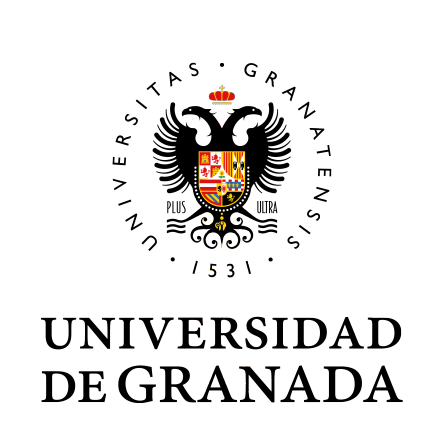
\includegraphics[scale=0.5]{img/ugr.png}\\

\textsc{\Large \asignatura{}\\[0.2cm]}
\textsc{GRADO EN INGENIERÍA INFORMÁTICA}\\[1cm]

\noindent\rule[-1ex]{\textwidth}{1pt}\\[1.5ex]
\textsc{{\Huge PROYECTO FINAL\\[0.5ex]}}
\textsc{{\Large Subtítulo práctica\\}}
\noindent\rule[-1ex]{\textwidth}{2pt}\\[3.5ex]

\end{minipage}

\vspace{0.5cm}

\begin{minipage}{\textwidth}

\centering

\textbf{Autores}\\ {\autor{}}\\{José María Sánchez Guerrero}\\[2ex]
\textbf{Rama}\\ {Computación y Sistemas Inteligentes}\\[2ex]
\vspace{0.3cm}


\includegraphics[scale=0.3]{img/etsiit.jpeg}

\vspace{0.7cm}
\textsc{Escuela Técnica Superior de Ingenierías Informática y de Telecomunicación}\\
\vspace{1cm}
\textsc{Curso 2018-2019}
\end{minipage}
\end{titlepage}

\pagenumbering{arabic}
\tableofcontents
\thispagestyle{empty}				% No usar estilo en la pagina de indice


\newpage

\setlength{\parskip}{1em}

\section{\textsc{Descripción del problema}}

El conjunto de datos con el que vamos a trabajar es el \textit{Image Segmentation Data Set}, creado por el Vision Group de
la Universidad de Massachusetts. Este conjunto de datos contiene una serie de características de casos extraídos al azar
de una base de datos con 7 tipos de imágenes tomadas al aire libre. Éstas imágenes fueron segmentadas manualmente para
crear una clasificación para cada píxel. Cada instancia es una región de $3 \times 3$.

Originalmente, nuestro conjunto de datos estaba ya dividido en training y test. Sin embargo, disponemos solo de 210 datos
de entrenamiento y 2100 de test. Como la cantidad de datos que tenemos para entrenamiento es muy inferior a la de test, y
no existe un motivo justificado por el que las particiones se hayan hecho de esta forma, hemos decidido juntar todos los
datos y crear nuestras propias particiones de entrenamiento y test. Esta división se comentará con más detalles en
secciones posteriores, cuando hablemos de las transformaciones y preprocesado que hemos realizado sobre los datos de los
que disponemos. 

Según la información proporcionada por la descripción del conjunto de datos, la cuál puede ser encontrada en el
repositorio UCI \cite{bib:uci-repo}, existen 7 clases distintas, y hay 30 muestras de cada clase en el conjunto de
entrenamiento y 300 en el conjunto de test. Con lo cuál, tenemos que en total hay 330 muestras de cada clase si miramos
los dos conjuntos de datos de forma conjunta. En total disponemos de 2310 muestras, cada una de las cuáles tiene 19
atributos que toman valores reales. En la representación original de los datos, tenemos que la primera columna se
corresponde con la clase de la muestra, y las 19 columnas restantes se corresponden con los atributos. 

De esta pequeña descripción podemos concluir que cada clase está idénticamente representada en los datos de los que
disponemos, y que no existe una clase que esté representada en mayor o menor medida que el resto de ellas. 

Con todo esto dicho, vamos a proceder a analizar cada una de las 19 características mencionadas anteriormente, para ver
que representa cada una de ellas:

\begin{enumerate}
	\item \textit{Region-centroid-col}: la columna del píxel central de la región.
	\item \textit{Region-centroid-row}: la fila del píxel central de la región. 
	\item \textit{Region-pixel-count}: el número de píxeles en una región. Su valor siempre es 9. 
	\item \textit{Short-line-density-5}: resultados de un algoritmo de extracción de rectas que cuenta cuántas líneas de longitud 5
	(con cualquier orientación) con bajo contraste, menor o igual a 5, cruzan la región. 
	\item \textit{Short-line-density-2}: igual que \textit{Short-line-density-5} pero cuenta con líneas de alto contraste,
	mayor que 5. 
	\item \label{it:vegde} \textit{Vegde-mean}: mide el contraste de píxeles horizontalmente adyacentes en la región. Hay 6 valores,
	pero se da dan la media y la desviación típica. Este atributo se utiliza como un detector de borde vertical. 
	\item \textit{Vegde-sd:} Desviación típica del contraste de píxeles horizontalmente adyacentes en la región (ver \ref{it:vegde}).
	\item \label{it:hedge} \textit{Hedge-mean}: mide el contraste de los píxeles verticalmente adyacentes.
	Utilizado para la detección de líneas horizontales. Este atributo es el valor medio.
	\item \textit{Hedge-sd}: Desviación típica del contraste de los píxeles verticalmente adyacentes (ver \ref{it:hedge}). 
	\item \textit{Intensity-mean}: el promedio sobre la región de (R + G + B) / 3.
	\item \textit{Rawred-mean}: Promedio sobre la región del valor R. 
	\item \textit{Rawblue-mean}: Promedio sobre la región del valor B. 
	\item \textit{Rawgreen-mean}: Promedio sobre la región del valor G. 
	\item \textit{Exred-mean}: Mide el exceso de rojo: (2R - (G + B)).
	\item \textit{Exblue-mean}: Mide el exceso de azul: (2B - (G + R)).
	\item \textit{Exgreen-mean}: Mide el exceso de verde: (2G - (R + B)).
	\item \label{it:value} \textit{Value-mean}: Transformación 3D no lineal de RGB.
	\item \textit{Saturatoin-mean}: (ver \ref{it:value}).
	\item \textit{Hue-mean}: (ver \ref{it:value}).
\end{enumerate}

Como estamos en un problema de clasificación, cada entrada produce una salida que es una etiqueta. La etiqueta puede hacer
referencia a una de las 7 clases que tiene el problema, las cuáles son: \textit{brickface}, \textit{sky},
\textit{foliage}, \textit{cement}, \textit{window}, \textit{path} y \textit{grass}. Para facilitar la representación de
las clases, vamos a transformar posteriormente cada valor de las etiquetas a un valor numérico. Esto se verá con más
detalle en secciones posteriores, cuando hablemos del preprocesado de los datos de entrada.

\newpage

\section{\textsc{Enfoque elegido para el análisis}}

El análisis y la elección de los modelos para nuestro problema va a tener varias fases, las cuales vamos a detallar a continuación:
\begin{itemize}[label=\textbullet]
\item Lo primero será el \textbf{preprocesado y análisis de los datos}, donde empezaremos leyendo los datos de los ficheros
proporcionados y los manipularemos para obtener un conjunto de datos con el que trabajaremos más cómodamente. Posteriormente se realizará
un estudio del conjunto de datos con la finalidad de conocer mejor el problema y cada uno de sus atributos y clases.
\item Después elegiremos las \textbf{métricas a utilizar}, donde seleccionaremos una serie de valores que nos permitan comparar los modelos.
Con una buena métrica podremos ver cómo de bueno es el rendimiento que nos ofrecen.
\item A continuación, \textbf{seleccionaremos los modelos a evaluar } y comentaremos brevemente cuáles son las \textbf{funciones de pérdida}
que utiliza cada modelo, además de comentar muy brevemente la aplicación de regularización a cada modelo.
\item Tras seleccionarlos tocará \textbf{evaluar y comparar los distintos modelos}, donde describiremos con más detalle la metodología
de evaluación seguida, probaremos los distintos modelos, analizaremos los resultados obtenidos y, a partir de ellos, compararemos el
rendimiento ofrecido por cada uno de ellos.
\item Una vez hayamos analizado los modelos, tendremos que \textbf{elegir y ajustar los mejores modelos}, donde utilizaremos los resultados
anteriores para seleccionar los que hayan funcionado mejor y luego ajustaremos sus hiperparámetros para intentar mejorarlos aun más.
\item Por último, vamos a \textbf{evaluar el mejor modelo}, es decir, una vez ajustados los mejores y decido cuál es el que nos va a resultar
más útil en nuestro problema, veremos como se enfrenta al conjunto de test. Analizaremos los resultados y concluiremos si hemos tomado una
buena decisión al elegir ese modelo.
\end{itemize}

\newpage

\section{\textsc{Preprocesado de los datos de entrada}}

En esta sección vamos a comentar el preprocesado que hemos hecho a los datos de entrada. Es decir, vamos a ver cómo y por qué juntamos
los dos conjuntos de datos y luego los separamos (tal y como dijimos en la sección anterior) y vamos a ver que modificaciones hacemos
sobre éstos para que nos sea más fácil trabajar posteriormente con ellos y para adaptarlos mejor al problema que queremos resolver.

Vamos a comenzar leyendo los datos y almacenándolos en estructuras de datos que nos permitan el fácil acceso a éstos. Posteriormente,
tal y como dijimos anteriormente, vamos a juntar los dos conjuntos en uno solo. Esto se puede ver a continuación:

\begin{lstlisting}
# Leer los datos de training y test
df1 = read_data_values('datos/segmentation.data')
df2 = read_data_values('datos/segmentation.test')

# Juntar los dos conjuntos en uno solo
df = pd.concat([df1,df2])
\end{lstlisting}

Nuestro objetivo al hacer esto es disponer de todos los datos de forma conjunta para luego poder crear nuestras propias particiones de
entrenamiento y de test, debido a que, como hemos dicho anteriormente, la cantidad de datos de entrenamiento de la que disponemos es
muy pequeña. Como no existe una justificación para no crear nuestras propias particiones, vamos a crearlas de tal forma que tengamos más
datos de entrenamiento que de test, conservando además la forma en la que cada clase está representada. Con esto, obtendremos un 
mejor modelo, ya que tendremos más datos con los que entrenarlo, y por tanto, va a generalizar mejor.

Sin embargo, antes de realizar las particiones, vamos a transformar las clases originales a valores numéricos, para que el trabajar
con ellas posteriormente sea más sencillo. Vamos a asignar a cada etiqueta un número. Como tenemos 7 clases, asignaremos un número
en el rango $[0, 6]$ a cada una de ellas, de forma que no se repita ningún número para ninguna etiqueta. Esta asignación se puede ver a
continuación:

\begin{lstlisting}
# Valor numerico asignado a cada etiqueta
labels_to_values = { 'BRICKFACE' : 0, 'SKY' : 1, 'FOLIAGE' : 2,
                     'CEMENT': 3, 'WINDOW' : 4, 'PATH' : 5,
                     'GRASS' : 6 }
\end{lstlisting}

Ahora ya solo nos quedaría aplicar el \textit{mapping}. Como todavía no hemos separado las etiquetas de los datos y sabiendo que, gracias
a la información proporcionada por el repositorio, la etiqueta se encuentra en la primera columna, la sustitución se puede hacer de forma
sencilla de la siguiente manera:

\begin{lstlisting}
# Sustituir etiquetas de salida por valores numericos discretos
df[0] = df[0].map(labels_to_values)
\end{lstlisting}

Con esto ya hecho, ya podemos dividir los datos en los valores de entrada $\mathcal{X}$ y las etiquetas $y$ y posteriormente dividir
éstos en los conjuntos de entrenamiento y de test. Queremos que el 80\% de los datos de los que disponemos esté en el conjunto de
entrenamiento y que el 20\% restante esté en el de test. Además, tal y como se mencionó anteriormente, queremos que las clases estén
igualmente representadas en los dos conjuntos en función de la cantidad de muestras que hay en total de cada clase. También es importante
mezclar los datos, con tal de que la elección de qué muestra va a cada conjunto no sea decidida por el orden de las muestras, si
no que se haga de forma aleatoria.

Se ha escogido esta repartición de los datos ya que nos permite tener un número suficientemente grande de muestras para entrenar nuestro
modelo y una cantidad aceptable de datos para ver como se desempeña con datos nunca vistos antes. La desventaja de hacer \textit{hold-out}
(que es lo que estamos haciendo aquí) es que perdemos datos para entrenar nuestro modelo, datos con los que, muy posiblemente, pudiésemos
obtener unos mejores resultados. Sin embargo, siguiendo este enfoque, tendremos al menos una forma de ver cómo de bien funciona nuestro
modelo con nuevos datos con los que nunca antes había interaccionado.

Vamos a ver ahora como se realizaría esta partición de los datos:

\begin{lstlisting}
# Obtener valores X, Y
X, y = divide_data_labels(df)

# Dividir los datos en training y test
# Conservar proporcionalidad de clase mezclando los datos
print('Splitting data in training and test sets...')
X_train, X_test, y_train, y_test = train_test_split(
        X, y, test_size=0.2, random_state=1, shuffle=True, stratify=y)
\end{lstlisting}

Y con todo esto visto, pasemos ahora a la parte de análisis de los datos, la cuál nos va a permitir obtener más información acerca de
los datos de los que disponemos.

\newpage

\section{\textsc{Análisis de los datos}}

En esta sección vamos a realizar un estudio de los datos para ver qué información nos pueden ofrecer sobre el problema. Lo primero que
vamos a hacer es observar algunas muestras del conjunto de entrenamiento para hacernos una idea de cómo es y qué valores pueden tomar
algunos de los atributos. Esto se puede ver a continuación:

\begin{figure}[H]
    \centering
    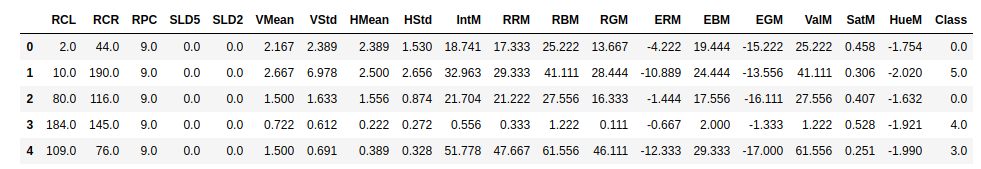
\includegraphics[scale=0.4]{img/train_df_head.png}
    \caption{Ejemplo del conjunto de datos de entrenamiento.}
    \label{fig:train-df}
\end{figure}

Una vez hecho esto, vamos a comprobar, para asegurarnos, cuáles son los tamaños de los conjuntos de entrenamiento y de test, y ver
si falta algún valor en estos conjuntos (a pesar de que en el repositorio se indicaba que no falta ninguno, nunca viene mal asegurarse).
Veamos a continuación qué información podemos extraer de aquí:

\begin{lstlisting}
# Determinar numero de muestras por conjunto
print('Training data size: ', train_df.shape[0])
print('Test data size: ', test_df.shape[0])

# Determinar si faltan valores para los dos conjunts
print('Missing values in train? ', train_df.isnull().values.any())
print('Missing values in test? ', test_df.isnull().values.any())
\end{lstlisting}

\begin{figure}[H]
    \centering
    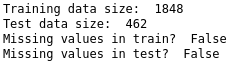
\includegraphics[scale=0.6]{img/df_info.png}
    \caption{Información sobre los tamaños de los conjuntos y la cantidad de valores que faltan.}
    \label{fig:train-test-stat}
\end{figure}

Podemos ver que el conjunto de entrenamiento tiene ahora 1848 muestras, mientras que el de test tiene 462. Estos nuevos tamaños son
resultado de la partición que hemos hecho anteriormente, y podemos ver claramente que el 20\% de los datos totales están en el
conjunto de test, tal y como habíamos especificado. Estos tamaños son más adecuados para entrenar los modelos, ya que al tener más
datos de entrenamiento, y si esta cantidad es lo suficientemente grande, los modelos podrán ser capaces de generalizar mejor. Como
al principio solo teníamos 200 datos de entrenamiento, la capacidad de generalizar de los modelos estaba más limitada. Aparte, tenemos
una cantidad de datos suficiente para poder probar luego nuestro modelo, para ver como se comporta con nuevos datos.

Pasemos ahora a estudiar un aspecto bastante importante de los datos que es la correlación de éstos. Nos interesa ver si existe
correlación lineal entre los datos de entrada y los de salida, para ver si sería necesario eliminar algún atributo. Además, también es
interesante ver si existe alguna correlación entre los atributos que tenemos como entrada. A continuación, se muestra la matriz de
correlación de los datos de entrenamiento, y sobre ella vamos a ir comentando los resultados:

\begin{figure}[H]
    \centering
    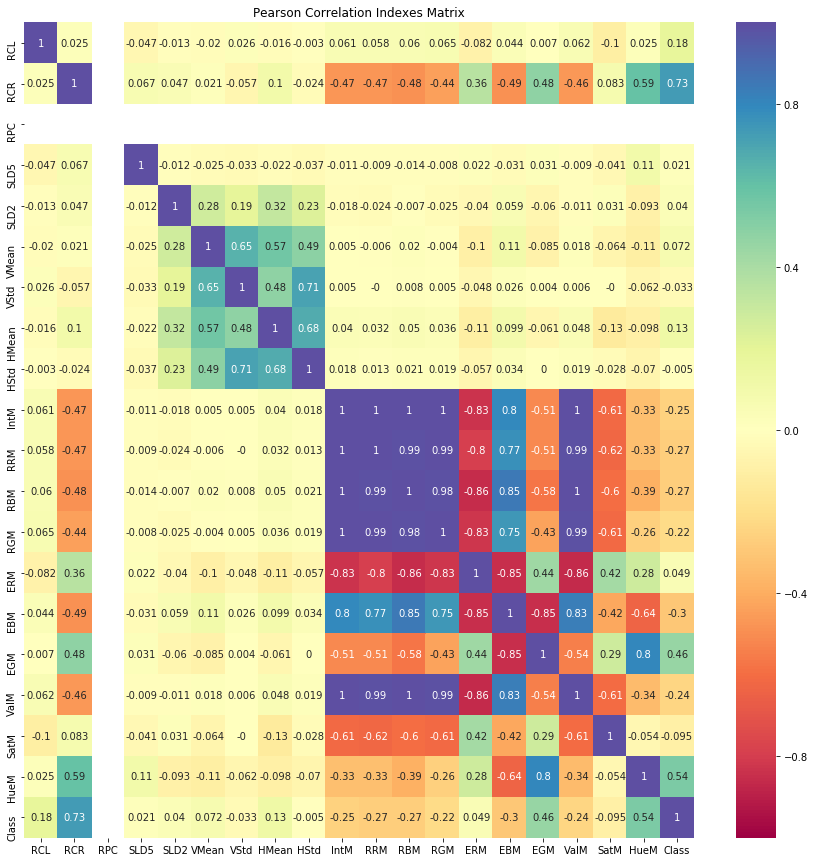
\includegraphics[scale=0.4]{img/correlation.png}
    \caption{Matriz con los coeficientes de correlación de Pearson.}
    \label{fig:pearson}
\end{figure}

De la figura anterior, podemos sacar algunas conclusiones:

\begin{itemize}[label=\textbullet]
    \item Tal y como nos indicaba la información del repositorio, existe un atributo que es constante, y que por tanto, no aporta
    ninguna información. Este atributo es el \textit{Region-pixel-count}, y se puede ver que en la figura no aparece ninguna
    información sobre éste. Por tanto, al ser un atributo ``inútil'', \textbf{va a ser eliminado}.
    \item Según lo que nos indica el gráfico, existen algunas variables que parecen tener una correlación mayor con la salida que
    otras. Por ejemplo, el \textit{Region-centroid-row} tiene una correlación de 0.73, un valor bastante alto. Sin embargo, al estar
    en un problema de clasificación, esta correlación no indica mucha información, ya que la salida es un valor discreto en vez de
    uno continuo, y por tanto, que la variable crezca o decrezca no parece indicar mucho en cómo va a afectar a la salida, ya que ésta
    es un valor discreto y no uno continuo.
    \item Existen una serie de variables de entrada que están bastante correlacionadas entre sí, ya que sus coeficientes de correlación de
    Pearson son 1, lo cuál significa que existe una correlación lineal entre ellas y que siempre que alguna de ellas crezca, la otra también
    lo hará. Esto nos podría indicar que podríamos eliminar algunos de estos atributos, ya que en un principio parecen aportar información
    redundante. Sin embargo, \textbf{no vamos a eliminar ninguna de las variables de entrada correlacionadas}, debido a que si decidimos
    eliminarlas a mano solo por tener una correlación lineal podríamos estar cometiendo un error, ya que nada nos asegura que esas variables
    no aportan información útil. Además, estaríamos tomando decisiones que podrían afectar posteriormente al modelo, y por tanto, sería
    mejor dejar que los modelos como tal decidan si esas variables son importantes o no en vez de hacerlo nosotros.
\end{itemize}

Con esto dicho, ya que hemos visto que existe una variable que no nos aporta ninguna información por el hecho de que es constante, vamos
a eliminarla tanto del conjunto de entrenamiento como el de test. Esto lo vamos a hacer a continuación mediante el siguiente código:

\begin{lstlisting}
# Crear lista de variables a eliminar
rm_list = [2]

# Eliminar variables de training y test
X_train = np.delete(X_train, rm_list, axis=1)
X_test = np.delete(X_test, rm_list, axis=1)
\end{lstlisting}

Habiendo eliminado esta variable, nos quedamos con 18 variables que vamos a utilizar en nuestro problema. Cada modelo ponderará a estas
variables de una forma u otra, dándoles diferente importancia.

Una vez concluido este pequeño análisis, vamos a pasar a comentar qué métricas vamos a utilizar para evaluar los modelos, antes de ver
exactamente cuáles de ellos utilizaremos.

\newpage

\section{\textsc{Elección de las métricas a utilizar}}

Está claro que, para comparar los distintos modelos y elegir a los mejores de entre ellos, necesitamos alguna métrica que nos permita
ver cómo de buenos son sus rendimientos. Como estamos en un problema de clasificación, parece que la \textit{accuracy} es una buena
elección, ya que es una métrica que indica cuántos elementos ha predicho el modelo correctamente sobre el número total de elementos. Además
de eso, la interpretación de esta métrica es muy sencilla e intuitiva, lo cuál no hace más que acentuar su idoneidad en este caso. Y,
aparte, es una muy buena métrica cuando el número de muestras que hay en cada clase está equilibrado, como es este caso, ya que los
resultados obtenidos son más representativos. En caso de no estar equilibradas, por ejemplo, si el 90\% de las muestras fuesen de una clase
y el 10\% fuese de otra, el clasificador podría tener una \textit{accuracy} de 90\%, pero podría estar clasificando correctamente solo
elementos de la clase predominante.

Con el modelo ya elegido, nos interesaría conocer algo más de información sobre su rendimiento, aparte de la \textit{accuracy}. Sería
interesante, por ejemplo, saber cómo clasifica con más detalle, viendo por ejemplo cuántos y qué elementos de cada clase clasifica
correctamente y en cuántos y cuáles de ellos se equivoca y en qué clase los clasifica. Esto se puede obtener mediante la
\textbf{matriz de confusión}. Esta matriz, además, nos permite obtener dos métricas más que tienen cierto interés.

Una de ellas es el \textit{recall} o sensibilidad, métrica que nos indica la proporción de elementos que pertenecen a una clase han sido
clasificados de forma correcta respecto al total de elementos que hay verdaderamente en esa clase. Esta métrica nos permite medir la
capacidad que tiene el clasificador de \textit{encontrar todas las muestras positivas}\cite{bib:recall}. Es decir, si tenemos que $TP$
(\textit{True Positives} o verdaderos positivos, a lo que se refiere con \textit{muestra positiva}) son los elementos de una clase
clasificados correctamente, y $FN$ (\textit{False Negatives} o falsos negativos) los elementos de una clase que han sido clasificados como
elementos de otra/s clases, tenemos que:

\[ 
\text{Recall} = \frac{TP}{TP + FN}
\]

La otra métrica es la \textit{precision} o precisión, la cuál nos indica qué proporción de elementos predichos de una clase se corresponden
a la clase real respecto a la cantidad total de elementos predichos de esa misma clase. Esta métrica nos permite medir la capacidad que tiene
el clasificador de \textit{no clasificar una muestra negativa como positiva}\cite{bib:precision}. Es decir, si tenemos que $TP$ son los
elementos de una clase clasificados correctamente, y que los $FP$ (\textit{False Positives} o falsos positivos, a lo que se refiere con
\textit{muestra negativa}) son los elementos que se han predicho que pertenecen a una determinada clase pero que en realidad pertenecen a
otra pertenecen a otra, tenemos que:

\[ 
\text{Precision} = \frac{TP}{TP + FP}
\]

De estas dos métricas, nos interesa obtener valores medios, ya que estamos en un problema de clasificación en el que hay múltiples clases.
Con lo cuál, nos interesa saber, de media, qué valores de \textit{recall} y \textit{precision} obtiene nuestro clasificador.

\section{\textsc{Elección de los modelos a evaluar}}

Una vez que hemos hablado de las métricas que vamos a utilizar para evaluar los distintos modelos, es hora de pasar a comentar la parte más
importante de todas, sin la cuál no tendría sentido nada de lo que estamos haciendo: los modelos. Hablaremos brevemente de qué modelos hemos
elegido y el por qué de cada uno de ellos.

\subsection{Regresión Logística Multinomial}

El primer modelo que hemos elegido es la Regresión Logística Multinomial, el cuál es un modelo lineal y es una generalización de la Regresión
Logística para múltiples clases. Esto último ha sido uno de los motivos principales por los que ha sido escogido, ya que permite trabajar con
múltiples clases, que es justamente lo que tenemos en este problema.

Existen otros muchos modelos que son variantes de la Regresión Logística para múltiples clases, como por ejemplo la Regresión Logística con
\textit{one-vs-rest}, donde se tienen $K$ modelos diferentes, donde $K$ es el número de clases. Cada modelo es un clasificador binario que
mide la probabilidad de que el elemento pertenezca a esa clase y la probabilidad de que el elemento no pertenezca a esa clase. Sin embargo,
en la Regresión Logística Multinomial hay un solo modelo que da $K$ probabilidades, las cuáles indican la probabilidad de que el elemento
pertenezca a cada una de las $K$ clases. Esto otra ventaja, ya que es mucho más intuitivo saber cuáles es la probabilidad real de pertenecer
a cada una de las $K$ clases para un dato de entrada.

La función de pérdida o \textit{loss function} que utiliza este modelo es la \textbf{Multi-class Cross Entropy}, una generalización de la
\textbf{Cross Entropy}, la cuál se utiliza en la Regresión Logística para dos clases. Esta función viene dada por la siguiente expresión:

\begin{equation}
\label{eq:mult-cross-entropy}
E(\mathbf{w_1}, \mathbf{w_2}, \dots, \mathbf{w}_K) = -\sum_{n=1}^N \sum_{k=1}^{K} y_{nk} \ln \Big(\sigma (\mathbf{w}_K^T \mathbf{x}_n)\Big)
\end{equation}

En cuanto a la regularización, como sabemos, nunca viene mal regularizar el modelo que estamos entrenando, ya que evitamos problemas de
\textit{overfitting} o sobreajuste, siempre y cuando el valor de $\lambda$ (hiperparámetro que pondera la regularización) sea el adecuado. 
En este caso, el modelo utilizará regularización de tipo $\ell 2$, debido a que la regularización $\ell 1$ se encargaría de eliminar ciertas
características asignándoles el valor 0, considerándolas como poco importantes. Al tener nosotros un número bastante pequeño de
características, no nos interesa mucho eliminar alguna de ellas, ya que podríamos perder información significativa.

\subsection{Support Vector Machine con \textit{kernel} RBF}

El segundo modelo que queremos evaluar es el SVM con \textit{kernel} RBF, un \textit{kernel} no lineal. Se ha escogido este \textit{kernel}
porque en general, en problemas de clasificación ofrece resultados bastante buenos y es bastante rápido. Hemos escogido este modelo porque,
aparte de encontrar una separación entre las clases, SVM también intenta buscar la separación óptima, dejando un margen suficiente a cada
lado, de forma que ningún punto caiga dentro de ese margen. Por tanto, está buscando también una separación \textbf{óptima} entre las clases.

Como muchas veces esto no es posible o los datos no son linealmente separables, se tienen que tolerar algunas violaciones de margen, dejando
que haya puntos dentro del margen o que no se hayan clasificado bien. Esto viene definido por el hiperparámetro $C$, el cuál indica cuál
es la importancia asociada a esta violación del margen. A menor peso, menos importancia, y por tanto, se consigue una separación más
regularizada y un margen más grande.

Este modelo funciona de forma diferente al SVM con \textit{kernel} lineal, ya que clasifica los datos por similaridad a los de la muestra.
Esta similaridad viene dada por la distancia euclídea. A mayor similaridad, menor la distancia. También está influida por un parámetro
$\gamma$, el cuál indica cuál es la influencia de ese punto. A mayor $\gamma$, menor influencia tendrán los puntos de la muestra, con lo cuál,
solo puntos muy cercanos a ellos podrán clasificarse como cercanos. A menor $\gamma$, más influencia tendrán los puntos de la muestra, y por
tanto, un nuevo punto podrá ser considerado como similar aún situándose bastante lejos del de la muestra. Este parámetro también define
cierto grado la regularización, ya que cuanto mayor sea el valor, mayor tendencia al sobreajuste, mientras que si es demasiado pequeño,
el modelo puede quedarse corto y sufrir de \textit{underfitting}.

La función de pérdida que utiliza este modelo, al igual que las otras variantes de SVM, es el \textbf{Hinge Loss}, el cuál tiene la siguiente
forma:

\begin{equation}
\label{eq:hinge-loss}
E_{SVM}(b, \mathbf{w}) = \frac{1}{N} \sum_{n=1}^N \max(1 - y_n \mathbf{w}^T\mathbf{x}_n + b , 0)
\end{equation}

\noindent la cuál no puede ser minimizada directamente al no ser derivable, si no que debe ser transformada y se debe resolver en el problema
dual.

En cuanto a la regularización, hay dos parámetros que influyen que se han comentado anteriormente, que son $\gamma$ y $C$. Por tanto, se
intentará controlar el parámetro $C$ a la hora de evaluar el modelo para hacer que no se obtenga un modelo muy ajustado a los puntos, y por
tanto, con sobreajuste.

\subsection{Random Forest}

El tercer modelo que queremos evaluar es el Random Forest, el cuál representa una mejora sobre los árboles de decisión clásicos y la técnica
de \textit{bagging}. Este modelo permite tener múltiples árboles de decisión los cuáles son entrenados cada uno con una muestra de datos
escogidos mediante \textit{bootsrap} de la original. Además, cada árbol escoge un subconjunto de predictores que va a utilizar para intentar
predecir, con el objetivo de evitar el problema de \textit{bagging} en el cuál la mayoría de árboles estaban correlacionados. Si
existe un predictor muy fuerte, este será utilizado casi siempre en la primera partición que se hace de los datos en cada árbol, haciendo por
tanto que la mayoría de árboles sea parecido.

Se ha escogido este modelo porque es un modelo que ofrece unos resultados muy buenos en general ya que tiene un bajo sesgo y una baja varianza
al tener múltiples árboles, que además no están correlacionados, lo cuál hace que la media de la varianza del modelo sea aún menor.

Como tal, la técnica de Random Forest no utiliza una función de pérdida, ya que no intenta minimizar nada. Sin embargo, sigue algún tipo de
heurística subyacente que permite construir el árbol con los datos de los que se dispone.

En cuanto a la regularización de este modelo, a pesar de que como tal ya ofrece una varianza baja, nunca está de más intentar hacer que
los árboles sean menos susceptibles al sobreajuste limitando la profundidad de éstos, por ejemplo (es decir, podando los árboles a priori).

\subsection{Redes Neuronales}

El último modelo que queremos evaluar son las Redes Neuronales. Concretamente, queremos probar un \textit{Multilayer Perceptron} o Perceptrón
Multicapa, el cuál es usado ampliamente en problemas de clasificación.

Hemos escogido este modelo ya que, en general, las Redes Neuronales permiten obtener unos resultados muy buenos en problemas complejos.
Como trabajan con capas de Perceptrones, se pueden conseguir separaciones de los datos en clases que con un Perceptrón simple nunca se
podrían conseguir, ofreciendo por tanto unos mejores resultados. Sin embargo, los tiempos de cómputo no acompañan a estos resultados, ya que
son modelos costosos desde el punto de vista computacional, además de que requieren una gran cantidad de datos. Sin embargo, consideramos que
la cantidad de datos de entrenamiento de la que disponemos después de crear nuestra propia partición de entrenamiento es suficiente, además
de que la arquitectura de la red no será muy compleja, en general.

La función de pérdida que utiliza este modelo es la misma que en la Regresión Logística Multinomial. Es decir, utiliza la \textbf{Multi-class
Cross Entropy}, la expresión de la cuál se puede ver en \eqref{eq:mult-cross-entropy}.

Aunque existan diversas técnicas de regularización como por ejemplo el \textit{early stopping}, hemos decidido no utilizar ningún tipo de
regularización a sabiendas de que existe cierto riesgo a que se produzca sobreajuste. Sin embargo, queremos ver su comportamiento sin
regularizar respecto a los otros modelos, para ver como se comportan.

\section{\textsc{Descripción del proceso de evaluación de modelos}}

Una vez vistos los modelos, vamos a pasar a ver cómo será la evaluación de éstos, describiendo el proceso seguido y las consideraciones que
se han tomado.

Para evaluar los distintos modelos, ya que queremos dejar el conjunto de test para el mejor modelo con tal de estimar su error fuera de la
muestra, podemos utilizar el conjunto de entrenamiento, y con él hacer un \textbf{10-fold cross-validation}. Es decir, podemos dividir
la muestra que tenemos en 10 particiones disjuntas del mismo tamaño o casi iguales (dependiendo de la cantidad de elementos de los que
dispongamos). Además, como estamos en un problema de clasificación, nos interesa que esos conjuntos disjuntos contengan un número proporcional
de elementos de cada clase respecto al número de elementos totales de cada clase que hay en el conjunto de entrenamiento original. De esta forma,
cada partición será una buena representación del conjunto de entrenamiento, y así, se evita que por ejemplo haya conjuntos que solo tengan
muestras de solo una clase, lo cuál podría producir resultados muy malos si el modelo nunca ha visto un ejemplo de ese tipo.

El motivo de escoger \textbf{cross-validation}

\section{\textsc{Evaluación y comparación de modelos}}

\begin{figure}[H]
    \centering
    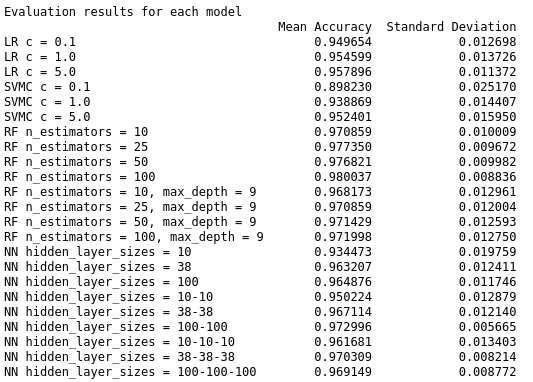
\includegraphics[scale=0.6]{img/eval-results.png}
    \caption{Resultado de la evaluación de los modelos.}
    \label{fig:eval-results}
\end{figure}

\begin{figure}[H]
    \centering
    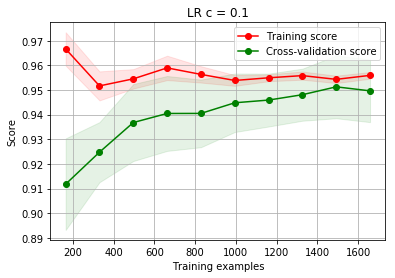
\includegraphics[scale=0.7]{img/lc-lr-c-01.png}
    \caption{Curva de aprendizaje del modelo de Regresión Logística con C=0.1.}
    \label{fig:lc-lr-c-01}
\end{figure}

\begin{figure}[H]
    \centering
    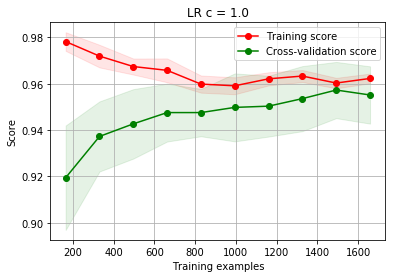
\includegraphics[scale=0.7]{img/lc-lr-c-1.png}
    \caption{Curva de aprendizaje del modelo de Regresión Logística con C=1.0.}
    \label{fig:lc-lr-c-1}
\end{figure}

\begin{figure}[H]
    \centering
    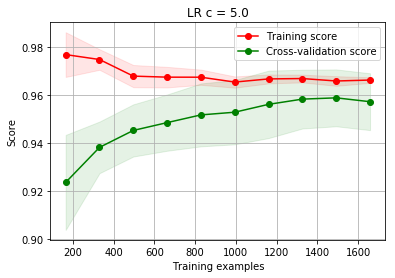
\includegraphics[scale=0.7]{img/lc-lr-c-5.png}
    \caption{Curva de aprendizaje del modelo de Regresión Logística con C=5.0.}
    \label{fig:lc-lr-c-5}
\end{figure}

\begin{figure}[H]
    \centering
    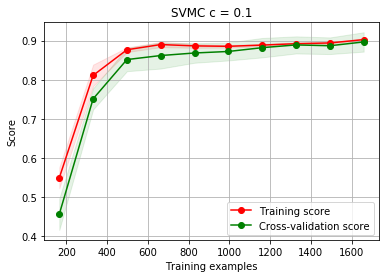
\includegraphics[scale=0.7]{img/lc-svm-c-01.png}
    \caption{Curva de aprendizaje del modelo SVM con C=0.1.}
    \label{fig:lc-svm-c-01}
\end{figure}

\begin{figure}[H]
    \centering
    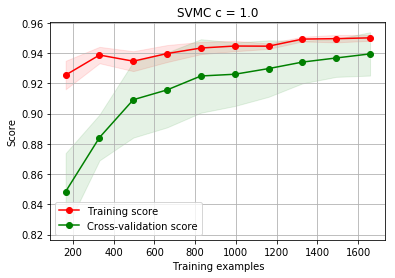
\includegraphics[scale=0.7]{img/lc-svm-c-1.png}
    \caption{Curva de aprendizaje del modelo SVM con C=1.0.}
    \label{fig:lc-svm-c-1}
\end{figure}

\begin{figure}[H]
    \centering
    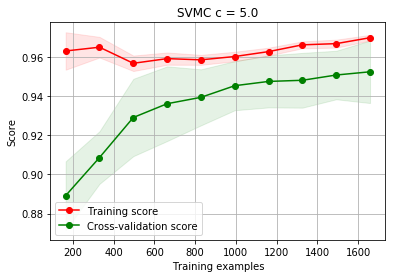
\includegraphics[scale=0.7]{img/lc-svm-c-5.png}
    \caption{Curva de aprendizaje del modelo SVM con C=5.0.}
    \label{fig:lc-svm-c-5}
\end{figure}

\begin{figure}[H]
    \centering
    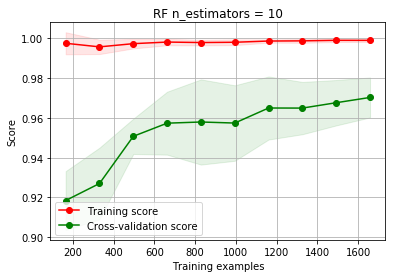
\includegraphics[scale=0.7]{img/lc-rf-n-10.png}
    \caption{Curva de aprendizaje del modelo Random Forest con $n\_estimators=10$.}
    \label{fig:lc-rf-n-10}
\end{figure}

\begin{figure}[H]
    \centering
    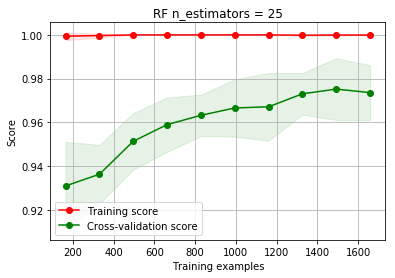
\includegraphics[scale=0.7]{img/lc-rf-n-25.png}
    \caption{Curva de aprendizaje del modelo Random Forest con $n\_estimators=25$.}
    \label{fig:lc-rf-n-25}
\end{figure}

\begin{figure}[H]
    \centering
    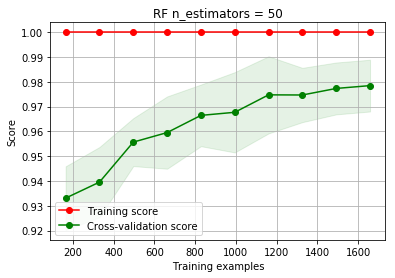
\includegraphics[scale=0.7]{img/lc-rf-n-50.png}
    \caption{Curva de aprendizaje del modelo Random Forest con $n\_estimators=50$.}
    \label{fig:lc-rf-n-50}
\end{figure}

\begin{figure}[H]
    \centering
    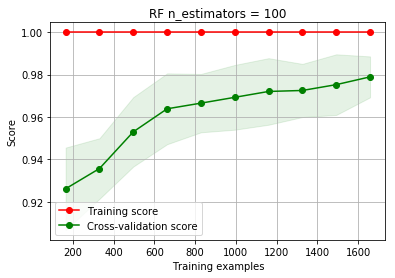
\includegraphics[scale=0.7]{img/lc-rf-n-100.png}
    \caption{Curva de aprendizaje del modelo Random Forest con $n\_estimators=100$.}
    \label{fig:lc-rf-n-100}
\end{figure}

\begin{figure}[H]
    \centering
    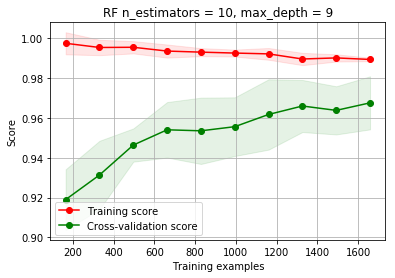
\includegraphics[scale=0.7]{img/lc-rf-n-10-d-9.png}
    \caption{Curva de aprendizaje del modelo Random Forest con $n\_estimators=10$ y $max_depth=9$.}
    \label{fig:lc-rf-n-10-d-9}
\end{figure}

\begin{figure}[H]
    \centering
    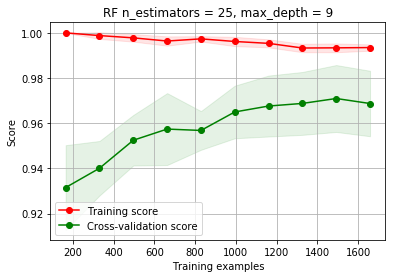
\includegraphics[scale=0.7]{img/lc-rf-n-25-d-9.png}
    \caption{Curva de aprendizaje del modelo Random Forest con $n\_estimators=25$ y $max_depth=9$.}
    \label{fig:lc-rf-n-25-d-9}
\end{figure}

\begin{figure}[H]
    \centering
    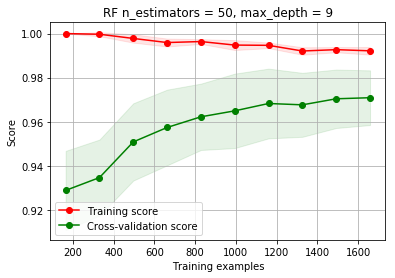
\includegraphics[scale=0.7]{img/lc-rf-n-50-d-9.png}
    \caption{Curva de aprendizaje del modelo Random Forest con $n\_estimators=50$ y $max_depth=9$.}
    \label{fig:lc-rf-n-50-d-9}
\end{figure}

\begin{figure}[H]
    \centering
    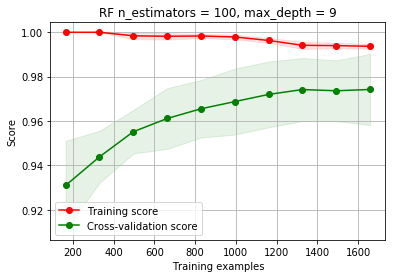
\includegraphics[scale=0.7]{img/lc-rf-n-100-d-9.png}
    \caption{Curva de aprendizaje del modelo Random Forest con $n\_estimators=100$ y $max_depth=9$.}
    \label{fig:lc-rf-n-100-d-9}
\end{figure}

\begin{figure}[H]
    \centering
    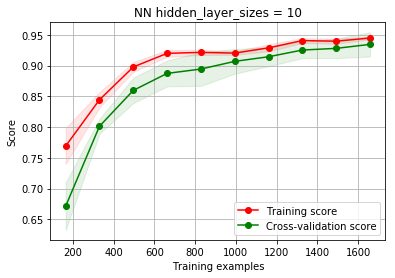
\includegraphics[scale=0.7]{img/lc-nn-10.png}
    \caption{Curva de aprendizaje del modelo de Neural Network con $hidden_layer_sizes=10$.}
    \label{fig:lc-nn-10}
\end{figure}

\begin{figure}[H]
    \centering
    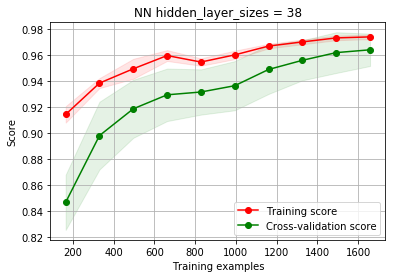
\includegraphics[scale=0.7]{img/lc-nn-38.png}
    \caption{Curva de aprendizaje del modelo de Neural Network con $hidden_layer_sizes=38$.}
    \label{fig:lc-nn-38}
\end{figure}

\begin{figure}[H]
    \centering
    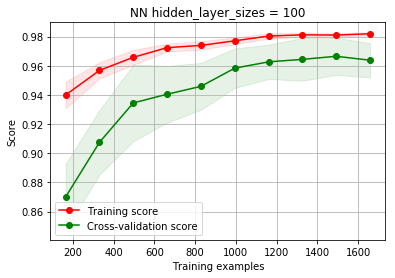
\includegraphics[scale=0.7]{img/lc-nn-100.png}
    \caption{Curva de aprendizaje del modelo de Neural Network con $hidden_layer_sizes=100$.}
    \label{fig:lc-nn-100}
\end{figure}

\begin{figure}[H]
    \centering
    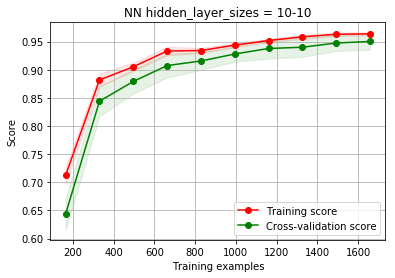
\includegraphics[scale=0.7]{img/lc-nn-10-10.png}
    \caption{Curva de aprendizaje del modelo de Neural Network con $hidden_layer_sizes=10-10$.}
    \label{fig:lc-nn-10-10}
\end{figure}

\begin{figure}[H]
    \centering
    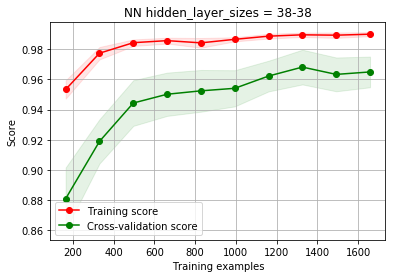
\includegraphics[scale=0.7]{img/lc-nn-38-38.png}
    \caption{Curva de aprendizaje del modelo de Neural Network con $hidden_layer_sizes=38-38$.}
    \label{fig:lc-nn-38-38}
\end{figure}

\begin{figure}[H]
    \centering
    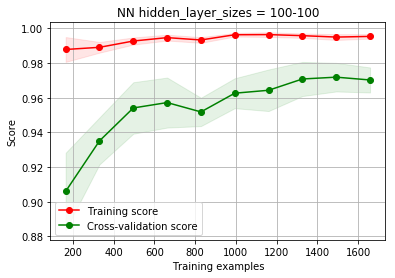
\includegraphics[scale=0.7]{img/lc-nn-100-100.png}
    \caption{Curva de aprendizaje del modelo de Neural Network con $hidden_layer_sizes=100-100$.}
    \label{fig:lc-nn-100-100}
\end{figure}

\begin{figure}[H]
    \centering
    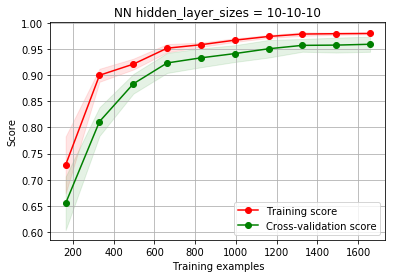
\includegraphics[scale=0.7]{img/lc-nn-10-10-10.png}
    \caption{Curva de aprendizaje del modelo de Neural Network con $hidden_layer_sizes=10-10-10$.}
    \label{fig:lc-nn-10-10-10}
\end{figure}

\begin{figure}[H]
    \centering
    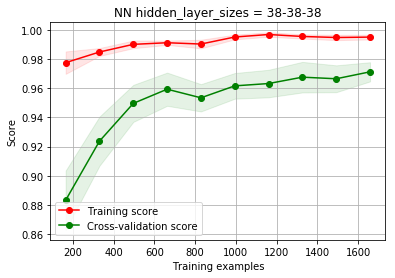
\includegraphics[scale=0.7]{img/lc-nn-38-38-38.png}
    \caption{Curva de aprendizaje del modelo de Neural Network con $hidden_layer_sizes=38-38-38$.}
    \label{fig:lc-nn-38-38-38}
\end{figure}

\begin{figure}[H]
    \centering
    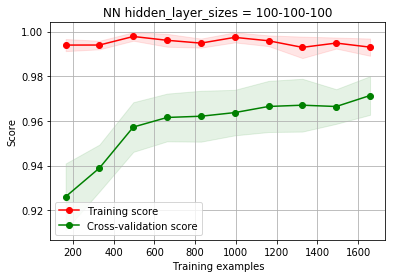
\includegraphics[scale=0.7]{img/lc-nn-100-100-100.png}
    \caption{Curva de aprendizaje del modelo de Neural Network con $hidden_layer_sizes=100-100-100$.}
    \label{fig:lc-nn-100-100-100}
\end{figure}

\newpage

\section{\textsc{Elección de los mejores modelos}}

Una vez analizados todos los modelos, utilizando \textbf{cross-validation} y diversos hiperparámetros para cada uno de ellos, vamos a
comentar cuáles han sido los que han obtenido los mejores resultados y porqué. Para ello nos vamos a ayudar de las métricas obtenidas
anteriormente, es decir, utilizaremos tanto la tabla que nos muestra la \textbf{media de aciertos} y \textbf{desviaciones típicas}, como
las \textbf{curvas de aprendizaje} de cada uno de los modelos (poner referencia a las tablas y gráficas).

Observando los resultados obtenidos, tenemos que el Random Forest con un $n\_estimators = 50$ es el que mayor porcentaje de acierto ha
tenido, con un 97.8470\%; mientras que el que menor desviación típica ha conseguido es el MLPClassifier con un $hidden\_layer\_sizes =
(100-100)$, con un valor de 0.005839. No obstante, podemos ver que el porcentaje de acierto de la mayoría de clasificadores es muy alto,
entre el 96\% y el 97\%, y los valores de las desviaciones típicas también son bastante bastante bajos, entre el 0.005 y el 0.02; así que
tendremos que tener en cuenta más cosas a parte de estas.

Vamos a analizar ahora las gráficas de los modelos para ver si encontramos algunos detalles más significativos en ellas:

\begin{itemize}[label=\textbullet]
\item Si empezamos por las de Regresión Logística, vemos que las curvas son bastante suaves  para los parámetros de $C = 1.0$ y $C = 5.0$ y a
medida que aumenta el número de evaluaciones, la clasificación va mejorando (aunque debido a la convergencia entre las dos líneas podemos
decir que, por más muestras de entrenamiento que tengamos, no va mejorar mucho mas) y el sobreajuste se reduce.

\item En cuanto al SVM, podemos ver que las gráficas no son malas, es decir, son bastante suaves y apenas tienen sobreajuste, pero los
resultados a
los que se está llegando son los peores en comparación con el resto.

\item En el Random Forest podemos ver que las curvas van aumentando suavemente a medida que el número de evaluaciones es más grande; y lo que es más importante, pueden seguir mejorando agregando más muestras de entrenamiento. Por otra parte, el valor del \textif{Training score} ronda siempre el 1, lo que puede causar sobreajuste.

\item Las gráficas de los MLPClassifier son muy similares a las del Random Forest, con la única diferencia de que los valores del
\textif{Training score} son mucho más parecidos a los que obtenemos en el \textif{cross-validation}. Esto quiere decir que, a diferencia del anterior, será más complicado que los problemas de sobreajuste aparezcan.
\end{itemize}
Gracias a este análisis, podemos decir que el SVM no va a ser uno de nuestros mejores modelos, porque nos ha ofrecido los resultados más
pobres en cuanto a la precisión y la desviación típica, y sus gráficas tampoco eran las mejores. Aun así, este no es un mal clasificador
(hemos podido comprobar que su porcentaje de acierto suele ser mayor de 90), pero lo tenemos que descartar porque tenemos al resto que
están un paso por delante.

Entre los tres modelos restantes nos vamos a quedar con la \textbf{Regresión Logística} y con el \textbf{Random Forest} por lo siguiente.
Los tres modelos han obtenido unos resultados muy buenos, incluso me atrevería a decir que el MLPClassifier tiene las mejores curvas de
aprendizaje y sólo superado en porcentaje de aciertos por algunos Random Forest, sin embargo, hemos descartado este clasificador porque es
mucho más complejo que los otros dos. Viendo los resultados, no hay una diferencia que sea lo suficientemente relevante como para elegir
este modelo, que es mucho más difícil y costoso en cuanto a tiempo de cómputo; frente a la rapidez y simplicidad de la Regresión Logística,
o frente al Random Forest que obtuvo los mejores resultados y que también es bastante más rápido.

\section{\textsc{Ajuste de las técnicas seleccionadas}}

\subsection{Regresión Logística}

Este modelo hemos visto que no ofrecía las mejores soluciones (aunque no se quedaba lejos de ellas), pero como es significativamente más
rápido que las redes neuronales, vamos a intentar ajustas sus hiperparámetros al máximo para conseguir mejorar sus resultados. Esto lo
haremos creando un grid con los distintos valores que le podremos asignar a nuestro algoritmo, y posteriormente ejecutándolo para cada uno
de ellos. Este es código que crea el grid y el modelo de Regresión Logística:

\begin{lstlisting}
# Crear grid de hiperparametros que se van a probar
param_grid_lr = [{'C': np.linspace(0.1, 1.0, 10),
                  'multi_class': ['multinomial'],
                  'solver': ['newton-cg'],
                  'random_state': [1]}]

# Crear modelo de regresion logistica
mlr = LogisticRegression()
\end{lstlisting}

Para el parámetro $C$ generamos una muestra de tamaño 10 con valores que van del 0.1 hasta el 1.0. Éste será el único hiperparámetro que
cambie, ya que $multi\_class$ sólo podrá adoptar el valor $'multinomial'$ y $solver$ sólo tendrán el valor $`newton-cg'$. El primero de
ellos es porque estamos en un problema multiclase, y el segundo de ellos porque ofrece una mejor minimización de la función cuadrática. El
último hiperparámetro $random\_state$ es la semilla para los aleatorios, así que no es muy importante.

A continuación, utilizaremos el método \textbf{\textit{GridSearchCV}}\cite{GridSearchCV} para realizar una búsqueda exhaustiva entre todos
los valores de los parámetros especificados y quedarnos con el mejor. Este método implementa funciones como $fit$ o $score$ que nos
ayudarán a evaluarlo, y parámetros como $best\_estimator\_$ que nos dirá cuál ha sido el mejor modelo de todos. Esta evaluación, al igual
que las anteriores, también se realizará mediante \textit{cross-validation} (implementada por la propia función). Veamos el código donde
aplicamos \textit{GridSearchCV}:

\begin{lstlisting}
# Crear GridSearch con Cross Validation para determinar
# la mejor combinacion de parametros
grid_search = GridSearchCV(mlr, param_grid=param_grid_lr, cv=cv,
                           scoring='accuracy')

# Aplicar GridSearch para obtener la mejor combinacion de hiperparametros
grid_search.fit(X_train, y_train)

# Obtener indice de la mejor media de test
best_idx = np.argmax(grid_search.cv_results_['mean_test_score'])

\end{lstlisting}

El resultado de ejecutar todo esto ha sido el siguiente:

\begin{figure}[H]
    \centering
    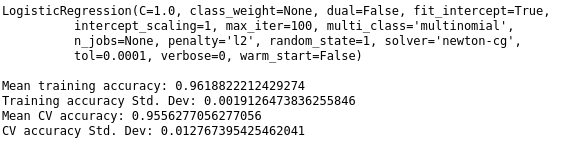
\includegraphics[scale=0.6]{img/gs-lr.png}
    \caption{Resultados de \textit{GridSearch} sobre la Regresión Logística.}
    \label{fig:gs-lr}
\end{figure}

Como podemos observar, el método ha seleccionado como valor para el hiperparámetro $C = 0.5$, el cual no habíamos prefijado en las pruebas
iniciales (0.1, 1.0, 5.0). Este valor está bastante bien estimado, ya que valores más bajos, como 0.1, hacen que la regularización sea muy
fuerte, mientras que con valores más altos, como 5.0, el sobreajuste aparecerá debido a que los errores tendrán una mayor penalización. Lo
lógico sería elegir valores por este rango de 0.5-1.0 aproximadamente, ya que son los que evitan los problemas anteriores.

Si nos paramos a analizar tanto la precisión como la desviación típica, los valores obtenidos con este nuevo hiperparámetro son peores, a
priori. Tenemos que tener en cuenta que este valor es calculado en $cross-validation$, y los valores más malos vienen a partir del tercer
decimal. Lo que nos lleva a decir que este modelo está mejor ajustado es que el valor de $C$ ha sido seleccionado de forma que se
regulariza en una medida apropiada para conseguir buenos resultados.

Concluimos que, pese a no haber mejorado los resultados iniciales, el modelo sigue clasificando bastante bien. No obstante, no lo
seleccionaríamos como el mejor modelo, ya que los clasificadores Random Forest lo hacen mejor con una complejidad similar (e incluso las
Redes Neuronales, aunque habría que estudiarlo en términos de eficiencia y simplicidad), y aún no hemos estudiado sus hiperparámetros y si
estos pueden hacer que mejore.

\subsection{Random Forest}

Es el turno de Random Forest, el modelo que mejores resultados ha obtenido en cuanto a precisión media y a varianza, que no tenía unas
malas curvas de aprendizaje, y que no es tan rápido como los SVM pero tienen una complejidad y tiempo de cómputo aceptable. Para intentar
mejorar, o encontrar los hiperparámetros que mejor se ajustan a este modelo vamos a utilizar la misma técnica de antes, el
\textit{GridSearchCV}. En este caso, el grid y el modelo Random Forest se crea de la siguiente forma:

\begin{lstlisting}
# Crear grid de hiperparametros que se van a probar
param_grid_rf = [{'n_estimators': np.linspace(50,500,10,dtype=np.int),
                  'max_depth': np.linspace(5, 15, 6, dtype=np.int),
                  'random_state': [1]}]

# Crear modelo de Random Forest
rf = RandomForestClassifier()

\end{lstlisting}

Para el hiperparámetro $n\_estimators$, que determina el número de árboles, generamos una muestra de tamaño 10 con valores que van desde el
50 hasta el 500; y para $max\_depth$, que determina la profundidad de los árboles, generaremos otra muestra, en este caso de tamaño 6 y con
valores que van desde el 5 hasta el 15. El último hiperparámetro también será $random\_state$, que al igual que antes, es la semilla para
los aleatorios.

Como la técnica para realizar la búsqueda de los mejores valores es la misma que la utilizada anteriormente en Regresión Logística, no la
vamos a volver a explicar, simplemente pasemos a ver los resultados que nos ha dado:

\begin{figure}[H]
    \centering
    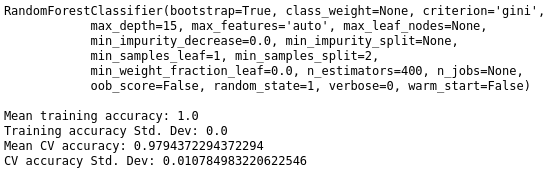
\includegraphics[scale=0.6]{img/gs-rf.png}
    \caption{Resultados de \textit{GridSearch} sobre Random Forest.}
    \label{fig:gs-rf}
\end{figure}

Podemos ver que el mejor valor que ha encontrado para el $n\_estimators$ ha sido 400, es decir, más alto (más número de árboles) que en el
modelo inicial, lo cual nos dice que tendríamos que haber probado con un número de árboles superior a  los prefijados. Por otro lado, para
$max\_depth$ el valor que ha obtenido ha sido 15, es decir, a diferencia de la ejecución inicial nos asigna un valor de profundidad límite.
También hay que tener en cuenta que nosotros intentamos poner una profundidad de 9 en esas ejecuciones y los resultados no eran tan buenos
como con estos hiperparámetros.

En cuanto a las medias en la precisión y en la desviación típica, también son valores muy similares a los obtenidos en la ejecución
inicial. Sin embargo, son valores similares a los árboles sin una profundidad determinada, es decir, que hemos conseguido un porcentaje de
acierto y una desviación típica tan buena como los anteriores pero con una profundidad de árbol limitada. También hay que tener en cuenta
el número de árboles utilizados, pero si se ha seleccionado este modelo como el mejor, es porque merece más la pena tener un mayor número
de árboles con una profundidad limitada que tener pocos árboles con mucha profundidad. Esto se debe a que los primeros se han podado a
priori y los segundos, al no haber especificado una profundidad máxima, no se han podado, con lo cuál son más sensibles al sobreajuste.

Como conclusión, decir que nos vamos a quedar con este último modelo de Random Forest obtenido como el mejor clasificador para el problema.
Ya vimos anteriormente que los Random Forest eran el mejor modelo (o de los mejores) en la ejecución inicial, y como acabamos de comprobar,
ajustando los modelos no hay ninguno que llegue a su nivel. Es más, ajustando el modelo hemos conseguido unos parámetros que mejoran los
asignados en un principio, así que partiremos de estos para realizar la evaluación final.

\section{\textsc{Evaluación del mejor modelo}}

Una vez elegido el modelo y ajustados los parámetros, vamos a realizar la evaluación final. Para ello nos ayudaremos de dos cosas: la primera es el \textbf{\textit{testing}} que no habíamos reservado al principio; y lo segundo es un modelo de referencia llamado \textbf{\textit{DummyClassifier}}\cite{DummyClassifier}, un modelo que utiliza reglas simples y que está especialmente diseñado para ser comparado con otras técnicas reales de clasificación (no se utiliza para problemas reales). El código para generar este clasificador es el siguiente:

\begin{lstlisting}
# Creamos modelo de prueba y lo entrenamos
dummy = DummyClassifier()
dummy.fit(X_train, y_train)

# Predecir valores con dummy
y_predicted_dummy = dummy.predict(X_test)
\end{lstlisting}

Podemos observar que estamos utilizando el clasificador con los parámetros por defecto. Entre estos tenemos uno llamado $strategy$, que por defecto tiene el valor $'stratified'$, el cual genera predicciones aleatorias respetando la distribución de clases del conjunto. Los otros dos atributos que tenemos son el $random\_state$, que ya vimos para que sirve, y otro llamado $constant$, que sólo afectará si el parámetro $strategy$ adopta un determinado valor (y no es nuestro caso).

Posteriormente, vamos a entrenar nuestro mejor modelo. Como estamos utilizando el que acabamos de ajustar y hemos clasificado como el mejor, no vamos a volver a explicar cómo se ha hecho. Simplemente, recordar que hemos utilizado un Random Forest con los hiperparámetros ajustados a 400 árboles con una profundidad máxima de 15.

A continuación, pasemos a la evaluación del modelo y a analizar los resultados obtenidos. Para ello vamos a mostrar las siguientes métricas para cada uno de los dos modelos: $accuracy$, $recall$ y $precision$. Lo realizaremos gracias a las siguientes líneas de código:

\begin{lstlisting}
# Obtener metricas
dummy_score = accuracy_score(y_test, y_predicted_dummy)
rf_score = accuracy_score(y_test, y_predicted_rf)

dummy_recall = recall_score(y_test, y_predicted_dummy,
                            average='macro')
rf_recall = recall_score(y_test, y_predicted_rf,
                         average='macro')

dummy_precision = precision_score(y_test, y_predicted_dummy,
                                  average='macro')
rf_precision = precision_score(y_test, y_predicted_rf,
                               average='macro')
\end{lstlisting}

Los parámetros que les pasamos son las etiquetas que esperamos obtener, las etiquetas que ha predicho cada uno de los modelos y, con $average$, el tipo de medias que obtendremos. En nuestro caso, con el valor $'macro'$, obtendremos la media estándar sin ponderar. Los resultados ha sido los siguientes:

\begin{figure}[H]
    \centering
    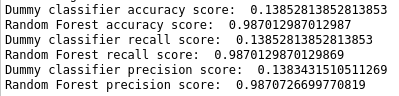
\includegraphics{img/model-comp-scores.png}
    \caption{Comparativa de métricas para evaluar el mejor modelo.}
    \label{fig:model-comp-scores}
\end{figure}

A simple vista nos damos cuenta de que un modelo aleatorio como el Dummy no es capaz de clasificar este problema correctamente. Podemos ver que ha obtenido unos resultados muy malos (simplemente con observar el $13\%$ aproximado para los tres parámetros a estudiar, ya nos dice que este problema tiene una complejidad a la hora de clasificar).

En cuanto a los resultados que ha obtenido el Random Forest, no tienen nada que ver con los del Dummy. Las predicciones han llegado a un $98.701\%$ tanto en \textit{accuracy}, como en \textit{recall} (es decir, la tasa de aciertos o tasa de verdaderos positivos), y como en \textit{precision} (verdaderos positivos entre todo el conjunto de positivos), y por tanto, comete un \textbf{$1.3\%$ de error}. Estos valores son mejores que los que obtuvimos anteriormente, al ajustar el modelo con \textit{cross-validation}. Esto es muy importante, ya que estamos comprobando que el ajuste lo hemos realizado correctamente y, pese que los resultados cuando lo evaluamos en su momento fueron peores, con un test más grande comprobamos que los hiperparámetros fueron elegidos correctamente.

Vamos a profundizar más en el análisis de este modelo sacando la matriz de confusión, para comprobar que parámetros obtenidos son correctos y dónde se han cometido los fallos:

\begin{figure}[H]
    \centering
    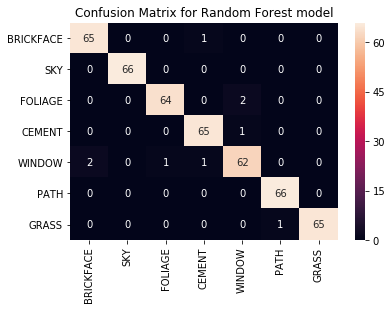
\includegraphics[scale=0.7]{img/confusion-matrix.png}
    \caption{Matriz de confusión de nuestro modelo ajustado.}
    \label{fig:confusion-matrix}
\end{figure}

Antes de analizarla, vamos a explicar que significa y que representa cada uno de sus valores. La matriz de confusión nos permite ver más detalladamente el rendimiento de un algoritmo a través de sus dos ejes. El horizontal que representa el número de predicciones para cada una de las clases; y el vertical, que representa los valores reales de las clases.

Si hubiésemos obtenido la matriz diagonal, el modelo tendría una precisión del $100\%$. En nuestro caso vemos que ha estado muy cerca de conseguirlo, ya que únicamente ha fallado en 6 de los 462 casos totales. Donde más ha fallado ha sido al clasificar las ventanas (\textit{WINDOW}), en la cuales ha puesto que 2 son ladrillos (\textit{BRICKFACE}) y una como cemento (\textit{CEMENT}). Esto quizás se deba a que la ventana esté situada en una pared de ladrillos u hormigón y el clasificador, al ver los parámetros de esta, lo haya entendido como tal. También encontramos un error al clasificar una tipo follaje (\textit{FOLIAGE}) como hierba (\textit{GRASS}), otro al clasificar una ventana (\textit{WINDOW}) como follaje (\textit{FOLIAGE}) y un último error al clasificar hierba (\textit{GRASS}) como cemento (\textit{CEMENT}).

Estos errores probablemente también se deban a la misma razón comentada anteriormente. Decimos esto porque, teniendo en cuenta que no hemos reducido dimensionalidad y tampoco hemos normalizado los datos (simplemente hemos eliminado una variable constante), el 'fallo' esté determinado por la propia imagen. Con esto nos referimos a que es un problema de la vida real, y los datos pueden contener ruido provocado, o bien, porque la imagen no sea lo suficientemente representativa, o porque simplemente necesitemos más atributos que nos permitan distinguir mejor entre clases.

Pese a comentar estos errores uno a uno no quiere decir que el modelo sea malo. Todo lo contrario, que hayamos podido enumerar los errores entre 462 datos nos da una idea de lo bien que ha clasificado y de los pocos errores que ha cometido.

Otra métrica que vamos a analizar sobre este modelo va a ser su \textit{curva de aprendizaje}. Vamos a ver primero la gráfica y posteriormente pasaremos a comentarla:

\begin{figure}[H]
    \centering
    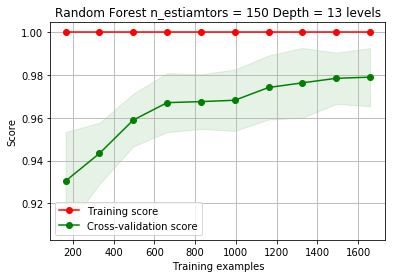
\includegraphics[scale=0.75]{img/lc-rf.png}
    \caption{Curva de aprendizaje de nuestro modelo ajustado.}
    \label{fig:lc-rf}
\end{figure}

Podemos ver que al principio, cuando tenemos pocos ejemplos de entrenamiento, la precisión entre los datos del \textit{Training} y del
\textit{Cross-validation} es muy diferente (tenemos una varianza muy alta). Sin embargo, a medida que vamos aumentando la cantidad de
ejemplos con los que entrenar, las líneas se empiezan a emparejar, ya que el modelo puede generalizar mucho mejor. La evolución de la curva
\textit{Cross-validation} es ascendente y bastante suave, lo que significa que el modelo aún tiene margen de mejora en caso de disponer de
más ejemplos de entrenamiento. El único inconveniente está en el sobreajuste debido a que, pese a tener curva muy buena como acabamos de explicar, la precisión de entrenamiento (siempre vale 1.0) es ligeramente mayor que en la validación.

\section{\textsc{Conclusiones}}

El objetivo de este trabajo era el de evaluar distintas técnicas para clasificar unas imágenes, extraídas del UCI Machine Learning Repository, según el tipo de material que veamos en ellas. Para realizar esta clasificación hemos dado los siguientes pasos.

Primero hemos analizado y modificado los datos, unificando los dos ficheros proporcionados, realizando nuestra propia división en \textit{training} y \textit{test}. Nos hemos dado cuenta de que no nos falta ningún valor en el conjunto y que nos sobra un atributo, que era constante para todos los datos. No hemos eliminado las correlacionadas para evitar eliminar información útil.

Hemos analizado todos los modelos, comentando cómo funcionan, sus funciones de pérdida, si utilizan regularización y cuál, y algunos detalles más específicos de cada uno. La evaluación de cada una de las técnicas la hemos realizado mediante las métricas \textit{accuracy}, \textit{recall} y \textit{precision}, y la técnica de validación cruzada a la hora de entrenar. Gracias a esto conseguimos un modelo que se ajuste de una forma generalizada a la naturaleza del conjunto de datos.

Cuando los hemos evaluado y comparado, nos hemos dado cuenta de que....

Las técnicas que hemos seleccionado como las mejores han sido \textbf{Regresión Logística} y \textbf{Random Forest}. La primera porque, con unos hiperparámetros prefijados por nosotros obtuvimos muy buenos resultados y no es una técnica tan compleja como las Redes Neuronales. Las Redes Neuronales obtuvieron mejor resultado, pero con una diferencia no lo suficientemente significativa como para compensar su complejidad. En cuanto al Random Forest, obtuvimos los mejores resultados sin apenas ajustar los modelos (únicamente probamos a limitar la profundidad a 9). Sus curvas de aprendizaje no eran las mejores, sin embargo, no es un modelo tan complejo como el anterior, así que merecía la pena intentar ajustarlo mejor.

Posteriormente, hemos ajustado estas dos técnicas mencionadas anteriormente. En Regresión Logística, hemos conseguido un mejor ajuste del parámetro C (con un valor de 0.5), que evita una fuerte regularización o que aparezca el sobreajuste. No obstante, en términos de precisión y desviación típica no ha mejorado al modelo inicial (95.5\% y 0.012 respectivamente), por lo que no lo seleccionaremos como el mejor. En cuanto al Random Forest, hemos conseguido ajustar un valor de profundidad $max_depth = 15$ pese a que el número de árboles que ha elegido es mayor al que asignamos inicialmente $n_estimators = 400$. Los valores de precisión y desviación típica son similares al modelo inicial (97.9\% y 0.010 respectivamente), aunque hay que tener en cuenta que los iniciales se obtuvieron sin una profundidad determinada.

Por último, hemos pasado a evaluar el mejor modelo (este último Random Forest que hemos comentado) a través del conjunto de test reservado al principio y un DummyClassifier. Gracias a esta evaluación y al posterior análisis, pudimos comprobar que, tanto la técnica elegida como el ajuste de sus hiperparámetros, lo hicimos bastante bien. Entre las 462 muestras sólo obtuvimos 6 errores. No podemos confirmar que esta sea la mejor técnica, pero gracias a todo este análisis, es bastante apropiado para resolver nuestro problema.

\newpage

% Pagina de bibliografia
\begin{thebibliography}{20}

\bibitem{bib:uci-repo}
UCI. \textit{Image segmentation}
\\\url{http://archive.ics.uci.edu/ml/datasets/image+segmentation}

\bibitem{logistic-regression}
Scikit-Learn. \textit{LogisticRegression}
\\\url{https://scikit-learn.org/stable/modules/generated/sklearn.linear_model.LogisticRegression.html}

\bibitem{svc}
Scikit-Learn. \textit{SVC}
\\\url{https://scikit-learn.org/stable/modules/generated/sklearn.svm.SVC.html#sklearn.svm.SVC}

\bibitem{random_forest}
Scikit-Learn. \textit{RandomForestClassifier}
\\\url{https://scikit-learn.org/stable/modules/generated/sklearn.ensemble.RandomForestClassifier.html#sklearn.ensemble.RandomForestClassifier}

\bibitem{neural_network}
Scikit-Learn. \textit{MLPClassifier}
\\\url{https://scikit-learn.org/stable/modules/generated/sklearn.neural_network.MLPClassifier.html#sklearn.neural_network.MLPClassifier}

\bibitem{scaler}
Scikit-Learn. \textit{StandardScaler}
\\\url{https://scikit-learn.org/stable/modules/generated/sklearn.preprocessing.StandardScaler.html}

\bibitem{pca}
Scikit-Learn. \textit{PCA}
\\\url{https://scikit-learn.org/stable/modules/generated/sklearn.decomposition.PCA.html}

\bibitem{learning_curve}
Scikit-Learn. \textit{plot\_learning\_curve}
\\\url{https://scikit-learn.org/stable/auto_examples/model_selection/plot_learning_curve.html#sphx-glr-auto-examples-model-selection-plot-learning-curve-py}

\bibitem{GridSearchCV}
Scikit-Learn. \textit{GridSearchCV}
\\\url{https://scikit-learn.org/stable/modules/generated/sklearn.model_selection.GridSearchCV.html}

\bibitem{DummyClassifier}
Scikit-Learn \textit{DummyClassifier}
\\\url{https://scikit-learn.org/stable/modules/generated/sklearn.dummy.DummyClassifier.html}

\bibitem{bib:recall}
Scikit-Learn. \textit{recall\_score}
\\\url{https://scikit-learn.org/stable/modules/generated/sklearn.metrics.recall_score.html}

\bibitem{bib:precision}
Scikit-Learn. \textit{precision\_score}
\\\url{https://scikit-learn.org/stable/modules/generated/sklearn.metrics.precision_score.html}

\end{thebibliography}

\end{document}

